The normal vector of the perpendicular line is
\begin{equation}
\begin{pmatrix}
7 \\
1
\end{pmatrix}       
\end{equation}
Thus, the desired equation of the line is 
\[
\begin{pmatrix}
7 & 1
\end{pmatrix}
\begin{pmatrix}
\vec{x} - 
\begin{pmatrix}
3 \\
0
\end{pmatrix}
\end{pmatrix} 
= 0
\]
\[
\Longrightarrow 
\begin{pmatrix}
7 & 1
\end{pmatrix}
\vec{x}
= 21
\]

See Fig.     \ref{fig:solutions_line_plane_37_a1}

\begin{figure}
    \centering
    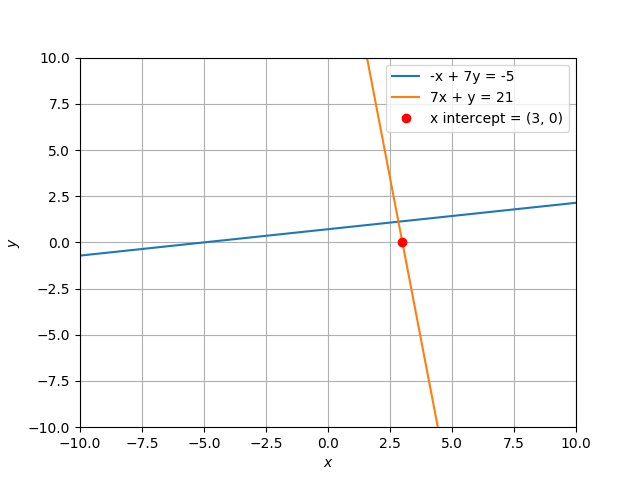
\includegraphics[width=\columnwidth]{solutions/line_plane/37/A1/a1.png}
    \caption{Plot showing intersection}
    \label{fig:solutions_line_plane_37_a1}
\end{figure}
